\documentclass[12pt,oneside]{article}
\usepackage[MeX]{polski}
\usepackage[utf8]{inputenc}
\usepackage{graphicx}
\usepackage[a4paper, total={170mm,257mm}, left=15mm, top=15mm]{geometry}
\linespread{1.25}
%\setlength{\parskip}{1ex plus 0.5ex minus 0.2ex}
\usepackage[hidelinks]{hyperref} 

% Title Page
\title{System CMS}
\author{Wojciech Korbecki\\ L2\\ 132768}
\date{}

\begin{document}
\clearpage\maketitle
\thispagestyle{empty}
\newpage
\tableofcontents

\section{Założenia aplikacji}
	\begin{itemize}
		\item Logowanie i rejestracja użytkownika do systemu
		\item Zmiana hasła użytkownika
		\item Przypomnienie hasła użytkownika
		\item Nadawanie grupom uprawnień
		\item Przypisywanie użytkowników do grup
		\item Pisanie wiadomości pomiędzy użytkownikami
		\item Tworzenie forum
		\item Pisanie wiadomości na forum
		\item Pisanie wiadomości na stronie głównej systemu
		\item Pisanie komentarzy
	\end{itemize}
\section{Technologie}
	Tworzony system został zahostowany na Hostinger.pl. W celu sprawdzenia systemu należy wejść na \url{http://wojciechk.hol.es}.
	\begin{itemize}
		\item PHP 5.5.35
		\item MariaDB 10.0.25
		\item Zend Framework 2.5.1
		\item Bootstrap
	\end{itemize}
\section{Konta użytkowników}
	Na potrzeby projektu zostały utworzone pięć kont, które każde posiada inne uprawnienia.
	\begin{itemize}
		\item \textbf{Zwykły użytkownik} \\
		Zwykły użytkownik posiada uprawnienia do przeglądania wiadomości na stronie głównej, przeglądania profilu swojego i innych użytkowników oraz do korespondencji z innymi użytkownikami.
		\begin{itemize}
			\item \textbf{Login:} user@user.pl
			\item \textbf{Hasło:} user
		\end{itemize}
		\item \textbf{Redaktor} \\
		Redaktor posiada te same uprawnienia co zwykły użytkownik oraz może tworzyć, edytować oraz usuwać wiadomości i komentarze.
		\begin{itemize}
			\item \textbf{Login:} news@news.pl
			\item \textbf{Hasło:} news
		\end{itemize}
		\item \textbf{Moderator forum} \\
		Moderator forum posiada te same uprawnienia co zwykły użytkownik oraz może tworzyć, modyfikować oraz usuwać fora i posty.
		\begin{itemize}
			\item \textbf{Login:} forum@forum.pl
			\item \textbf{Hasło:} forum
		\end{itemize}
		\item \textbf{Administrator} \\
		Administrator posiada te same uprawnienia co zwykły użytkownik oraz może tworzyć, modyfikować oraz usuwać użytkowników.
		\begin{itemize}
			\item \textbf{Login:} admin@admin.pl
			\item \textbf{Hasło:} admin
		\end{itemize}
		\item \textbf{Właściciel} \\
		Właściciel posiada wszystkie wymienione wcześniej uprawnienia.
		\begin{itemize}
			\item \textbf{Login:} root@root.pl
			\item \textbf{Hasło:} root
		\end{itemize}
	\end{itemize}
\section{Harmonogram}
\begin{tabular}{|c|c|c|}
	\hline \textbf{Nazwa zadania} & \textbf{Data rozpoczęcia} & \textbf{Data zakończenia} \\ 
	\hline Logowanie i rejestracja & 01-11-2016 & 05-11-2016 \\ 
	\hline Panel administratora & 10-11-2016 &  \\ 
	\hline System newsów & 10-11-2016 & 05-12-2016 \\ 
	\hline System komentarzy & 10-11-2016 & 08-01-2017 \\
	\hline System zarządzania użytkownikami & 08-12-2016 &  \\ 
	\hline System korespondencji pomiędzy użytkownikami & 08-12-2016 &  \\ 
	\hline Forum & 01-01-2017 &  \\ 
	\hline 
\end{tabular} 
\section{Diagram ERD}
	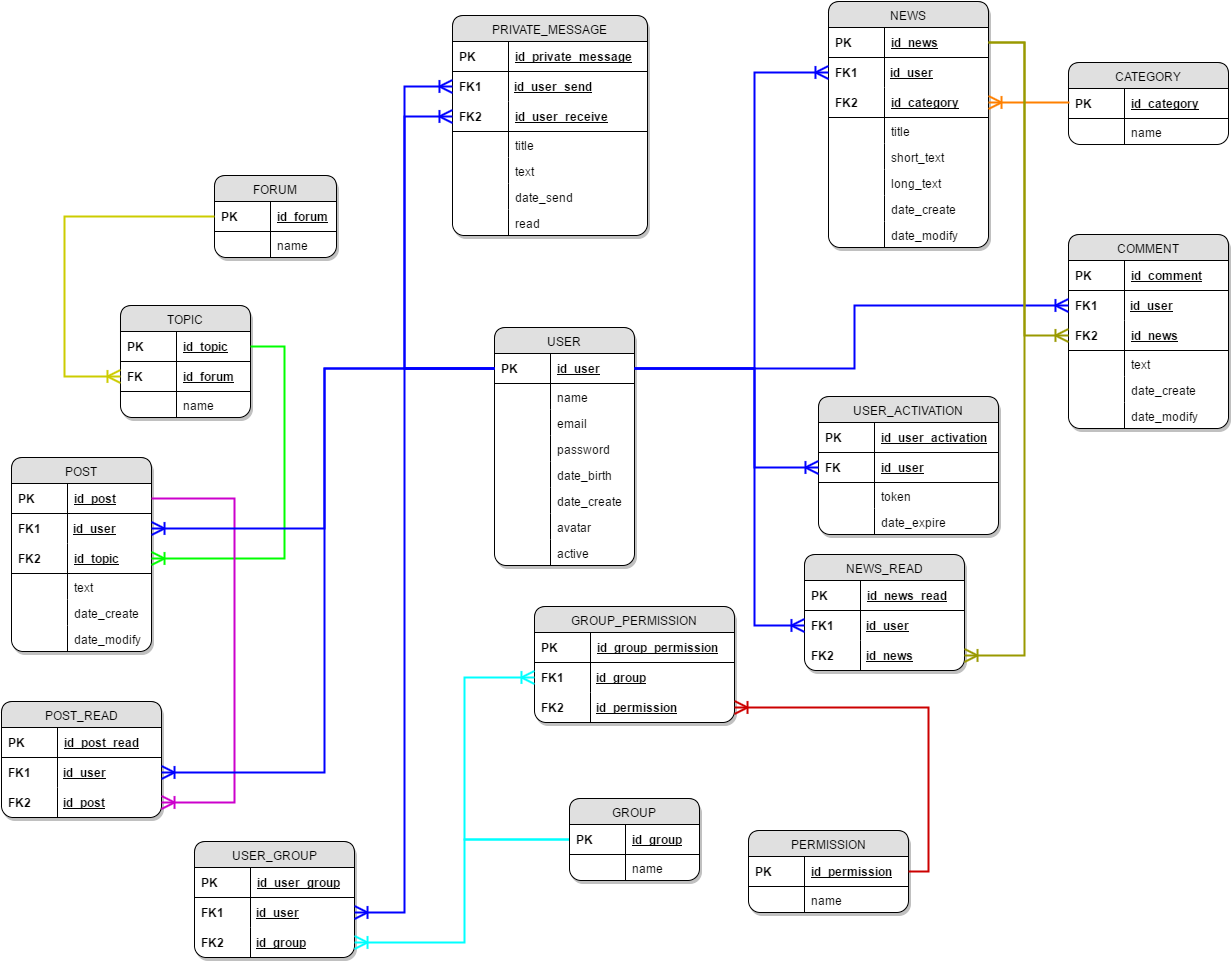
\includegraphics[width=1\textwidth]{erd3.png}
\end{document}          
